\begin{figure}[htbp]
\centering
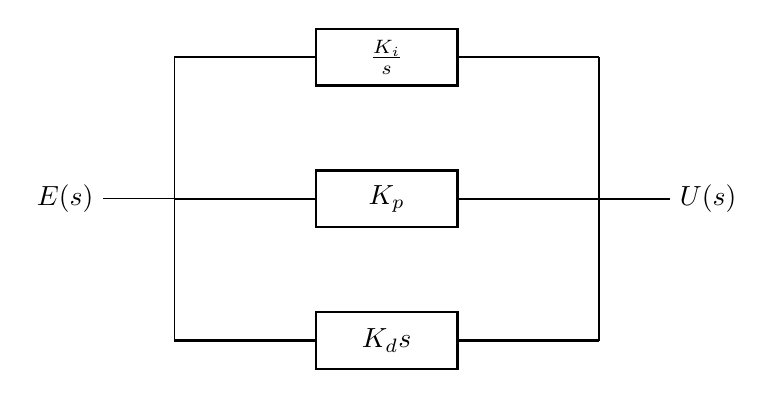
\begin{tikzpicture}[scale=0.9]
    % Input
    \node[left] at (-1,0) {$E(s)$};

    % Summing junction
    \draw[-] (-1,0) -- (0,0);

    % Three parallel paths
    \draw[-] (0,0) -- (0,2);
    \draw[-] (0,0) -- (0,-2);

    % P path
    \draw[thick] (0,0) -- (2,0);
    \draw[thick, fill=white] (2,-0.4) rectangle (4,0.4);
    \node at (3,0) {$K_p$};
    \draw[thick] (4,0) -- (6,0);

    % I path
    \draw[thick] (0,2) -- (2,2);
    \draw[thick, fill=white] (2,1.6) rectangle (4,2.4);
    \node at (3,2) {$\frac{K_i}{s}$};
    \draw[thick] (4,2) -- (6,2);

    % D path
    \draw[thick] (0,-2) -- (2,-2);
    \draw[thick, fill=white] (2,-2.4) rectangle (4,-1.6);
    \node at (3,-2) {$K_d s$};
    \draw[thick] (4,-2) -- (6,-2);

    % Summing
    \draw[thick] (6,2) -- (6,0);
    \draw[thick] (6,-2) -- (6,0);
    \draw[thick] (6,0) -- (7,0);

    % Output
    \node[right] at (7,0) {$U(s)$};
\end{tikzpicture}
\caption{PID controller block diagram.}
\label{fig:pid_block}
\end{figure}
